
% !TeX root=DeepRelAttr.tex
% !TEX TS-program = pdfLatex

%%%%%%%%%%%%%%%%%%%%%% INTRODUCTION %%%%%%%%%%%%%%%%%%%%%%%%%%%%%%
\section{Introduction}

%  After the "Relative Attributes" paper \cite{parikh2011}, there was a stream of papers that aimed to solve the same or similar task (\cite{Li2013,Yu2014,Sandeep_2014_CVPR,Lee_2013_7540}) using a different and often more complex model instead of the original RankSVM model. I think as progress in the "Visual Recognition" field has shown, for solving the problem you actually need to change the features not the model. So in this project I actually want to experiment with how learning the features end-to-end (or fine-tuning the features) can improve Relative Attributes accuracy and power. 
 
%  Please follow the notations as in here\footnote{\notation}. We will remove this footnote. I just put it here, so that we all know how to write the formulations. Use \



Visual attributes are linguistic terms that bear semantic properties of (visual) entities, often shared among categories. They are both human understandable and machine detectable, which makes them appropriate for better human machine communications. Visual attributes have been successfully used for many applications, such as image search \cite{pubfig, whittlesearch}, interactive fine-grained recognition \cite{branson10, branson13} and zero-shot learning \cite{6571196, parikh2011}.

Traditionally, visual attributes were treated as binary concepts \cite{ferrari2007learning, Farhadi09describingobjects}, as if they are present or not, in an image or a scene. Parikh and Grauman ~\cite{parikh2011} introduced a more natural view on visual attributes, in which pairs of visual entities can be compared, with respect to their relative strength of any specific property. With a set of human assessed relative orderings of image pairs, they learn a global ranking function for each attribute (Figure \ref{fig.1}).
While binary visual attributes relate properties to entities (\eg, a dog being furry), relative attributes make it possible to relate entities to each other in terms of their properties (\eg, bunnies being furrier than dogs).

\begin{figure}
\centering
\scalebox{.3}
{
\begin{tikzpicture}
	% pair 1
	\node (p1A) {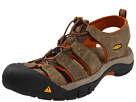
\includegraphics[scale=0.65]{Fig1/pair1A.jpg}};
	\node (p1op) [right=0.0cm of p1A, scale=3] {$>$};
	\node (p1B) [right=-0.4cm of p1op] {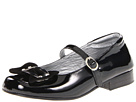
\includegraphics[scale=0.65]{Fig1/pair1B.jpg}};

	\draw[line width=2, rounded corners] ($(p1A.north west)+(-0.0,0.5)$)  rectangle ($(p1B.south east)+(0.0,-0.5)$);
	
	% pair 2
	\node (p2B) [right=0.0cm of p1B] {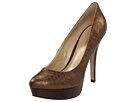
\includegraphics[scale=0.65] {Fig1/pair2B.jpg}};
	\node (p2op) [right=0.0cm of p2B, scale=3] {$<$};
	\node (p2A) [right=-0.4cm of p2op] {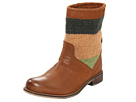
\includegraphics[scale=0.65] {Fig1/pair2A.jpg}};

	\draw[line width=2, rounded corners] ($(p2B.north west)+(0.2,0.5)$) rectangle ($(p2A.south east)+(0.0, -0.5)$);

	% dots
	\node (dots) [right=0.1cm of p2A, scale=4] {\dots};

	% pair3
	\node (p3A) [right=0.0cm of dots] {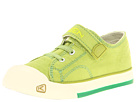
\includegraphics[scale=0.65]{Fig1/pair3A.jpg}};
	\node (p3op) [right=0.0cm of p3A, scale=3] {$>$};
	\node (p3B) [right=-0.4cm of p3op] {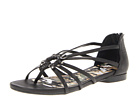
\includegraphics[scale=0.65]{Fig1/pair3B.jpg}};

	\draw[line width=2, rounded corners] ($(p3A.north west)+(-0.2,0.5)$) rectangle ($(p3B.south east)+(0.2, -0.5)$);

	% Training phase box and label	
% 	\draw[line width=2, rounded corners, red, loosely dotted] ($(p1A.north west)+(-0.4, 1)$) rectangle ($(p3B.south east)+(0.4, -1)$);

% 	\path (p1A.north east) -- (p3B.north west) node [scale=3, above=1cm, pos=0.5] {Training};

	% bottom mid point
	\path (p1A.south east) -- (p3B.south west) node (mid) [below=1cm, pos=0.5] {};

	% testing pair
	\node (uop) [below=4cm of mid, scale=4] {$?$};
	\node (puA) [left=0.5cm of uop] {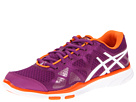
\includegraphics[scale=1]{Fig1/pairUA.jpg}};
	\node (puB) [right=0.5cm of uop] {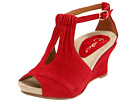
\includegraphics[scale=1]{Fig1/pairUB.jpg}};
	
	\draw [line width=2, rounded corners, dashed] ($(puA.north west)+(-0.2, 0.5)$) rectangle ($(puB.south east)+(0.2, -0.5)$);
	
	% testing phase arrow
	\path [draw, ->, line width=10] (mid.south) -- ($(uop.north) + (0cm, 2cm)$);	

\end{tikzpicture}}
\caption{Visual Relative Attributes. This figure shows samples of training pairs of images from the UT-Zap50K dataset, comparing shoes in terms of `comfort' (top). The goal is to compare a pair of two novel shoe images, respective to the same attribute (bottom).}
\label{fig.1}
\end{figure}

Many have tried to build on the seminal work of Parikh and Grauman \cite{parikh2011} with more complex and task specific models for ranking, while still using hand crafted visual features, such as GIST \cite{Aude01} and HOG \cite{hog}. Recently, Convolutional Neural Networks (ConvNets) have proved successful in various visual recognition tasks, such as image classification \cite{krizshevsky}, object detection \cite{RCNN} and image segmentation \cite{fullyconv}. Many attribute the success of ConvNets to their ability to learn multiple layers of visual features from data. 

In this work, we propose to use a ConvNet-based architecture to learn the ranking of images, using relatively annotated images for each attribute. Pairs of images with similar and/or different strengths of some particular attribute are presented to the network. The network  learns a series of visual features, which are known to work better than engineered visual features \cite{offtheshelf}. After learning the features, we further propose to add another layer to the network, to rank the images. The ranking layer could be learned through gradient descent (described in more details later). As a result, it would be possible to learn (or fine-tune) the features through back-propagation, while learning the ranking layer. Interweaving the two processes leads to a set of learned features that characterize each single attribute. This escalates the overall performance and is the main advantage of our proposed method over previous methods. Furthermore, in almost all previous works on relative attributes, the training phase often can only handle inequality relations (\ie, one image being less or more strong, in terms of a specific attribute, than the other). The equality relation can happen quite frequently when humans are qualitatively deciding about the relations of attributes in images. In previous works this is not explored, even in some, the equality relation could not be incorporated in the training phase, due to method limitations. Our proposed method introduces an easy and elegant way to deal with equality relations (\ie an attribute is similarly strong in two images).
%%%%%%%%%%%% spatial extent shall be removed from the paper
%It is noteworthy to pinpoint that by exploiting the saliency maps of the unsupervised learned features for each attribute, similar to \cite{simonyan14a}, we can discover the spatial extent \cite{specialextent} of the attribute. %This is done using the same network in an unsupervised manner.
%%%%%%%%%%%% spatial extent shall be removed from the paper

Our approach achieves very competitive results and improves the state-of-the-art (with a large margin in some datasets) on {\it all} major publicly available datasets for relative attributes, both coarse-grained and fine-grained.

% (we might need to save some space.) No need for this:  (If we had extra space, we can put it back... )
The rest of the paper is organized as follows: Section \ref{sec.2} discusses the related works. Section \ref{sec.3} illustrates our proposed method, including the ConvNet for learning the feautres and the ranking layer. Then, Section \ref{sec.4} exhibits the experimental setup and results, and finally, Section \ref{sec.5} concludes the paper.
